
\chapter{Supplementary Notes}
  \label{SuppNotes}

\section{Measurement Techniques}
  \subsection{MAX-DOAS}
    Multiple axis DOAS (MAX-DOAS) is a remote sensing technique which uses several DOAS measurements over different viewing paths.
    In these retrievals, the measurements of light absorption are performed over several elevations in order to add some vertical resolution to the measurement of trace gas concentrations.
    An example of this is shown in figure \ref{LR:HCHO:fig_MAXDOASExample}, which was taken from \textcite{Lee2015}.
    Recently MAX-DOAS has been used to examine HCHO profiles in the clean free troposphere (\textcite{Franco2015, Schreier2016}) as well as in polluted city air (\textcite{Lee2015}).
    Depending on orography and atmospheric composition (ie. the influence of interfering chemicals), MAX-DOAS can be used to split the tropospheric column into two partial columns; giving a small amount of vertical resolution to HCHO measurements \parencite[eg.]{Franco2015, Lee2015}.
    In \textcite{Franco2015}, an FTIR spectrometer at Jungfraujoch is compared against both MAX-DOAS and satellite data, with two CTMs; GEOS-Chem and IMAGES v2 used to compare total columns and vertical resolution of each instrument.
    
    \begin{figure}
      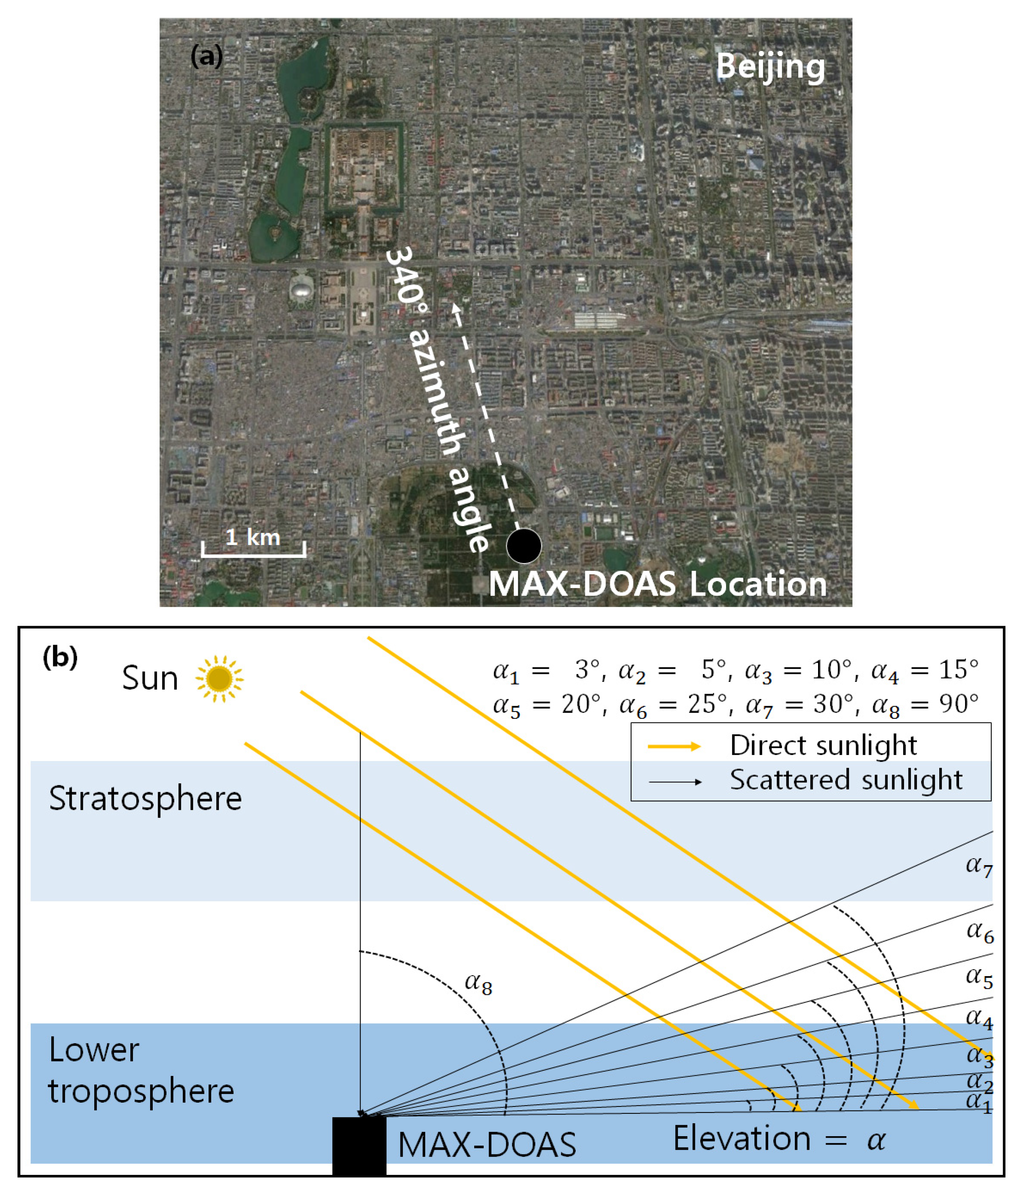
\includegraphics[width=\textwidth]{Figures/MAXDoasExample.png}
      \caption{ Image from \textcite{Lee2015}.}
      \label{LR:HCHO:fig_MAXDOASExample}
    \end{figure}

\section{Data sets}
  \subsection{SPEI}
    
    The Standardised Precipitation Evapotranspiration Index (SPEI) is a measure of drought using TODO \textcite{SPEI_website}.
    This product covers 1901 - 2011, and uses the average over that period as the background, in order to compare drought stressed regions against those with sufficient or excess water \textcite{SPEI_website}.

\section{Chemistry}
  
  \textcite{Patchen2007} examine the branching step where isoprene either forms ROO or RONO$_2$, and for specific conditions they determine the reaction rates for each branch.
  They find the most frequent pathway is the formation of ROO (99.3\%).
  Although the nitrates formation is relatively infrequent, this pathway can lead to NO$_X$ transport into clean environments \parencite{Horowitz1998}.
  This transport can be exacerbated by fast winds and low OH concentrations, making nitrates an important factor in modelling atmospheric chemistry.
  
  PAN has a relatively long lifetime (against OH, order of 1 day) and is able to transport and release the NO$_X$ in environments which are quite far from any emissions.
  
  \subsubsection{SOA}
    \label{LR:VOCs:IsopCascade:SOA}
    
    SOA formation from VOCs in atmospheric CTMs is generally imperfect due to the complicated chemistry and diverse nature of atmospheric conditions.
    Yields of SOA from VOCs are often lumped together and based on empirical laboratory chamber data. 
    VOC oxidation was not feasible $\sim 13$ years ago (2005), as chamber studies did not extend over a large enough parameter range and the importance of heterogeneous aerosol chemistry on SOA formation was unquantified \parencite{Kanakidou2005}.
    
    
    %% SOA production and overview?
    Gas phase emissions with higher vapour pressures can be oxidised into lower vapour pressure products which will partition between gas and particle phase, often called semi or non-volatile. 
    The aerosol products from these gas phase emissions (or the children thereof) are called SOA \parencite{Kanakidou2005}.
    In the \cite{Kanakidou2005} review of global SOA science, uncertainty in radiative forcing of aerosols is highlighted, and 20-90~\% of PM mass in the lower troposphere is OA.
    Less volatile OA also plays a role, although PM production from this source is complicated and makes up only a small fraction ($\sim 1 \%$) of the resulting PM (\cite{Kroll2008, Bei2012}).
    Modelling OA has many uncertainties due to the complexity of SOA formation and various pathways such as aqueous phase oxidation which can significantly contribute to concentrations.
    This is further hindered by poor understanding of precursor emissions, and lumping together various compounds, of which only some form SOA (for example ORVOCs in GEIA (back in 2005)).
    Satellite data requires SOA models to estimate a full vertical profile of aerosols for remote sensing techniques \parencite{Kanakidou2005}.
    
    SOA formation from VOCs in atmospheric CTMs is generally imperfect due to the complicated chemistry and diverse nature of atmospheric conditions.
    Yields of SOA from VOCs are often lumped together and based on empirical laboratory chamber data. 
    VOC oxidation was not feasible $\sim 13$ years ago (2005), as chamber studies did not extend over a large enough parameter range and the importance of heterogeneous aerosol chemistry on SOA formation was unquantified \parencite{Kanakidou2005}.
    
    One of the large uncertainties with OA is the total effect on radiative forcing, 12 years ago it was well understood that most OA cool the atmosphere, with smaller particles having a larger affect due to the size matching the wavelengths of visible light \parencite{Kanakidou2005}. 
    Transport and indirect effects complicate matters further, with cloud creation and modification of cloud properties being quite difficult to accurately predict.
    In the third IPCC report \parencite{IPCC2001}, the uncertainty involved if OA forcing was a factor of 3 times the estimated effect. 
    This has since been improved however OA and cloud formation still remains a large uncertainty in more recent IPCC reports \parencite{IPCC_Chapter2}.
    Figure \ref{LR:VOCs:IsopCascade:SOA:fig_IPCC_RF_AR4} shows the radiative forcing (RF) of various atmospheric constituents, it's clear that OA uncertainty dominates.
    Figure \ref{LR:VOCs:IsopCascade:SOA:fig_IPCC_RF_AR5} shows the same summary updated in chapter 8 of the fifth report, where the SOA uncertainty remains quite large.
    It's currently understood that SOA plays an indirect and complex role in cloud properties, with a net cooling effect \parencite[Chapter 7,8]{IPCC_AR5_WG1}
    
    \begin{figure}
      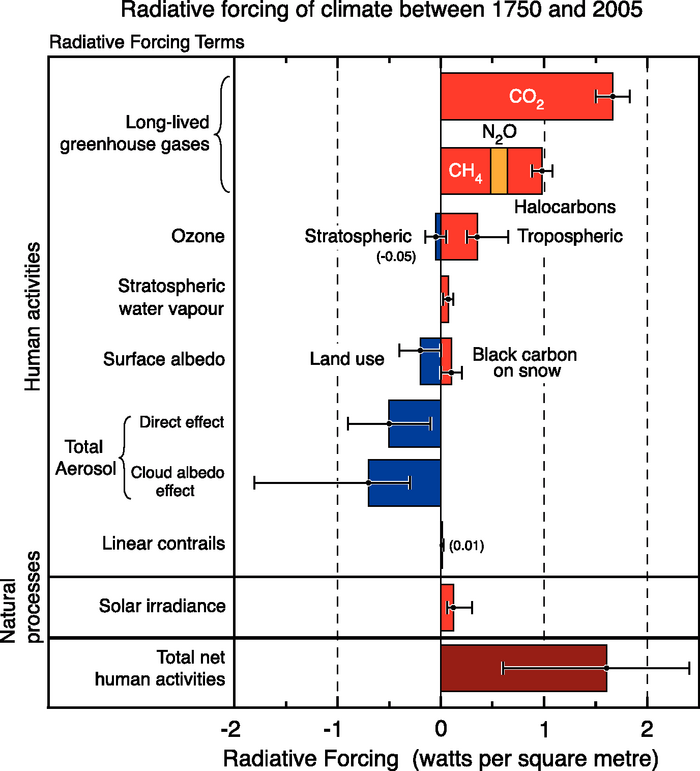
\includegraphics[width=\textwidth]{Figures/IPCC_WG1AR4_RFSummary.png}
      \caption{%
        The overall radiative forcings and uncertainties of several atmospheric constituents
        This is an image taken from \cite{IPCC_Chapter2}, found at \url{https://www.ipcc.ch/publications_and_data/ar4/wg1/en/faq-2-1.html}.}
      \label{LR:VOCs:IsopCascade:SOA:fig_IPCC_RF_AR4}
    \end{figure}
    
    \begin{figure}
      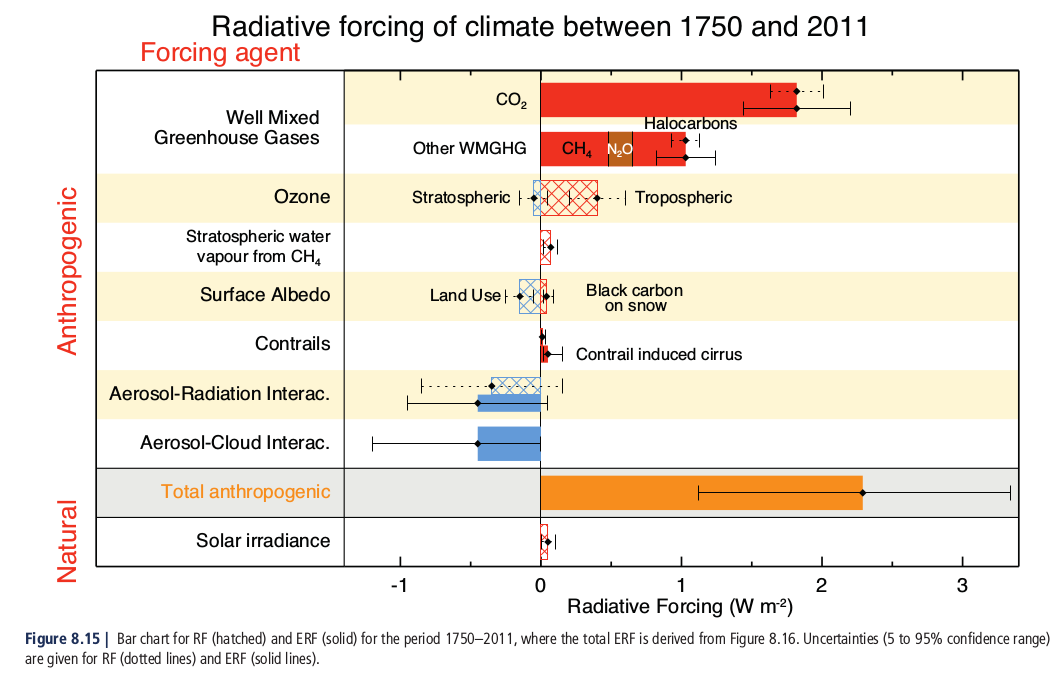
\includegraphics[width=\textwidth]{Figures/IPCC_WG1AR5_RFSummary.png}
      \caption{%
        The overall radiative forcings and uncertainties of several atmospheric constituents
        This is an image taken from \cite{IPCC_AR5_WG1}, chapter 8.}
      \label{LR:VOCs:IsopCascade:SOA:fig_IPCC_RF_AR5}
    \end{figure}    
    
    (TODO: read more of Kanakidou2005)
    The emissions of precursors to SOA was and is quite uncertain, in \cite{Kanakidou2005} they state that these uncertainties range from a factor of 2 to 5.
    They highlight emissions and flux measurements as well as implementing satellite data in models as a means of improving the emissions inventories.
    In 2005, (as of \cite{Kanakidou2005},) the knowledge gaps in isoprene and terpene oxidation processes included precursor gases to SOA, impact of NO$_X$ on SOA formation, heterogeneous reactions between particles and gaseous compounds, aqueous phase chemistry, and complete aerosol compositions.
    At this time SOA driven nucleation was under debate, as chamber studies showed that SOA led to new particles but only in the particle free laboratory setting. 
    Nucleation of new particles was suppressed by condensation if any seed aerosol was already present.
    Observed nucleation outside of laboratories was suggested to have arisen from biogenic SOAs, driven by ozonolysis.
    \cite{Kanakidou2005} concluded that it is very likely that organics contribute to particle growth and formation rates.
    
    \cite{Rollins2009} examine SOA production in a large chemical reaction chamber, over 16~hr in the dark and find first generation mass yield ($\Delta$SOA mass$/\Delta$isoprene mass) to be less than 0.7\%, with further oxidation of initial products (isoprene reacting twice with NO$_3$) yielding 14\%.
    This led to an overall mass yield of 2\% over the 16~hr experiment.
    Night NO$_3$ levels also affect O$_3$, TODO: millet et al 2016. %TODO: millet 2016
    
  \subsection{Relationship to Glyoxyl TODO: remove if never used}
    
    Another chemical retrievable from satellite observation is Glyoxyl, which can be used to further determine what sort of precursors to HCHO are being emitted \parencite{Stavrakou2009, Miller2014, Miller2017}.
    TODO: go through 2014 paper and see if it's easy to retrieve, then email Dr. Chris Miller.
    For example \cite{Cao2018_discuss} recently used Glyoxyl measurements to improve understanding of biogenic and anthropogenic NMVOC emissions over China.
    This involved using a method pioneered by \cite{Stavrakou2009} TODO: get this cite and check method out.
    
    Glyoxyl (CHOCHO) is important to us as it shares many properties with HCHO, and may provide additional information in determining isoprene emissions.
    Glyoxyl is another product of VOC oxidation in the atmosphere, with isoprene being the main source globally.
    Under high NO$_X$ conditions, glyoxyl forms rapidly, similarly to HCHO.
    However, glyoxyl also forms in low NO$_X$ environments both slowly (through isoprene epoxydiols), and rapidly (through di-hydroperoxide dicarbonyl compound photolysation \parencite{Crounse2013}.
    This process is similar to the proposed mechanisms for hydroperoxyaldehydes by \cite{Peeters2014} and carbonyl nitrates \parencite{Muller2014}.
    Aromatics which are largely anthropogenic form glyoxyl quickly, while HCHO is produced slower, allowing determination of anthropogenic sources \parencite{Cao2018_discuss}.
    
    HCHO has been used to estimate isoprene emissions (some examples in Section \ref{LR:HCHO:SatelliteInversion}) but many uncertainties exist.
    One of these uncertainties is the yield of HCHO from isoprene, especially in low NO$_X$ environments.
    Glyoxyl could prove complementary to HCHO in constraining isoprene emissions (TODO: Read and cite Vrekoussis2009,2010, Chan Miller 2014, Alvarado 2014) \parencite{Miller2017}.
    Recently \cite{Miller2017} updated GEOS-Chem to include the prompt formation of glyoxyl and compared this with satellite and airplane measurements over the USA.
    With coming geostationary satellites, which provide greater time resolved measurements of HCHO and CHOCHO, this mechanism could be used to clearly show when low NO$_X$ isoprene chemistry is being undertaken \parencite{Miller2017}.
    
  
\section{CAABA/MECCA}
  \label{Model:CM}
  
  
  CAABA (Chemistry As A Boxmodel Application) estimates the chemical concentrations accounting for J-values (JVAL), simplified and parameterised photolysis (SAPPHO) and simplified emission and depositions (SEMIDEP).
  CAABA runs in a single scenario (or box) with given emissions, depositions, and initial concentrations, allowing the examination of chemistry in a very specific environment to be modelled with high temporal resolution.
  CAABA/MECCA has been implemented for various calculations including ozone chemistry throughout the atmosphere in \cite{Zanis2014}.
  The user manual is available online at \url{http://www.rolf-sander.net/messy/mecca/caaba_mecca_manual.pdf}.
  
  This has been used with an atmospheric chemistry model MECCA (Module Efficiently Calculating the Chemistry of the Atmosphere) which implements tropospheric and stratospheric chemistry for both the gas and the aqueous phases \parencite{Sander2005}.
  MECCA chemical mechanisms include basic O$_3$, CH$_4$, NO$_X$, and HO$_X$ chemistry, as well as non methane hydrocarbon (NMHC) chemistry, considering gas phase, aqueus phase, and heterogenous reactions. \parencite{Sander2005}
  For the numerical integration, MECCA uses the KPP software (\cite{SanduSander2006}), which takes chemical reactions and their rate coefficients and codes integral solutions to the system.
  The combination of the CAABA box model with MECCA module is called CAABA/MECCA and is currently at version 3.
  CAABA/MECCA been implemented for various calculations including ozone chemistry throughout the atmosphere in \cite{Zanis2014}.
  
  MECCA could also be used as the chemistry mechanism for a more complex, 3-dimensional model (\cite[e.g.][]{Jockel2006}).
  The connection is established via the MESSy interface (\url{http://www.messy-interface.org}) developed by \cite{Jockel2005} as part of an effort to simplify the framework for modelling the atmospheres at various scales.
  The user manual is available online at \url{http://www.rolf-sander.net/messy/mecca/caaba_mecca_manual.pdf}.
  
  \subsubsection{CAABA/MECCA outputs}
  The box model can output in netcdf or text format, TODO: which way am I better off ? 
  Text output from CAABA/MECCA was read using tailored python scripts modified from code written by dr. Luke Surl.
  Dr. Luke Surl also wrote the code which implements calculations of yield from runs using isoprene injections as described in Section \ref{Model:CM} TODO: update to more specific reference.
  
  % Method for using caaba/mecca
  \subsection{CAABA/MECCA Box model: isoprene source classifications}
    \label{BioIsop:Methods:CM}
    
    %% HOW WE WILL USE CAABA/MECCA
    Using CAABA/MECCA to examine isoprene to HCHO yield in specific scenarios allows us to determine what environment may be driving the yield calculated by GEOS-Chem.
    Initially we have three scenarios, grassland, desert, and forest Australia - with each scenario having initial conditions, emission and deposition set as in table TODO:\ref{}.
    Running each scenario with and without a small isoprene injection allows calculation of isoprene lifetimes and HCHO yield for those scenarios.
    
    CAABA runs in a single scenario (or box) with given emissions, depositions, and initial concentrations, allowing the examination of chemistry in a very specific environment to be modelled with high temporal resolution.
    This has been used with an atmospheric chemistry model MECCA (Module Efficiently Calculating the Chemistry of the Atmosphere) which implements tropospheric and stratospheric chemistry for both the gas and the aqueous phases \parencite{Sander2005}.
    For our purposes it's worth noting that MECCAs chemical mechanism includes basic O$_3$, CH$_4$, NO$_X$, and HO$_X$ chemistry, as well as non methane hydrocarbon (NMHC) chemistry, considering gas phase, aqueus phase, and heterogenous reactions. \parencite{Sander2005}
    For the numerical integration, MECCA uses the KPP software \parencite{SanduSander2006}, which takes chemical reactions and their rate coefficients and forms efficient code for integral solutions to the system.
    The combination of the CAABA box model with MECCA module is called CAABA/MECCA and is currently at version 3.
    
    
    %TODO: Description of how scenario yields can be calculated.
    We perscribe parameters values approximating three seperate (and relatively broad) scenarios: forest, urban, and scrubland.
    These parameters are shown in Table \ref{BioIsop:table:CAABAMECCA_Scenarios}!
    The initial concentrations, the influx, (TODO: check this) and the deposition rates of various chemical species or families is perscribed.
    Chemical creation, destruction and deposition rates are determined every X minutes.
    This is done by altering a scenarios file which does not change over the lifetime (TODO: 40 days?) of the model runs.
    For each scenario, two nearly identical model runs are performed, one with an injection of isoprene occuring on (TODO: when/howmuch is this injection).
    The concentrations of isoprene and HCHO for our three scenarios, with and without the isoprene injection, is plotted over time in figure TODO: CAABA/MECCA scenario figures.
    The yield of HCHO from isoprene is then calculated by looking at the difference between each parallel run to determine how much of the injected isoprene transformed into HCHO.
    Isoprene life time can also be calculated using this process, as the time it takes for the extra isoprene to reach $1/e$ of it's initial value.
    
    %% CALCULATION OF YIELD
    TODO: Calculations for this (from Luke, double check these and enter them here).
    Calculation of the yield follows a calculation of the theoretical maximum carbon production by the amount of injected isoprene:
    \begin{equation}
    Y_{100} =10^9 \times \frac{C_{PM} E_{inj} D_{inj}}{(N_A H_{PBL})}
    \end{equation}
    Where Y$_{100}$ is the maximum possible carbon yield of isoprene (ppb), $C_{PM}$ is Carbon per molecule (isoprene=5), $E_{inj}$ is the emission rate of injected isoprene (molec cm$^{-2}$ s$^{-1}$), $D_{inj}$ is the duration of injection (s), H$_{PBL}$ is the boundary layer height (cm), and $N_A$ is the Air number density (molec cm$^{-3} \approx 2.5e19$).
    Finding the accumulated increase in HCHO (ppb) from the difference between the perturbed and non perturbed model runs allows calculation of the accumulated extra HCHO (Example: Figure TODO:), which divided by the $Y_{100}$ gives us the isoprene to HCHO atom C yield:
    \begin{equation}
    Y_{HCHO}= \frac{\Delta HCHO_{\text{Accumulated}}}{Y_{100}}
    \end{equation}
    with $HCHO_{\text{Accumulated}}$ being the accumulated enhanced ppb mixing ratio of HCHO.
    
    Figure TODO: shows the accumulated yield for all three scenarios, which each increase towards a limiting value.
    
    \begin{table}[t]
      \caption{Parameters for each scenario used in CAABA/MECCA model runs. TODO: fill these values in}
      %    Parameter | S1, S2, S3
      \begin{tabular}{ c |  c   c   c  } 
        \hline
        Parameter(units) 		 & Forest & Scrublands & Urban\\
        \hline
        Initial concentrations & & & \\
        NO$_X$(molec cm$^{-3}$)		 & low  & low  & high \\
        O$_3$(molec cm$^{-3}$)  & mid & mid & low \\
        HO$_X$(molec cm$^{-3}$) & & & \\
        \hline 
        Influx & & & \\
        NO$_X$(molec cm$^{-3}$ s$^{-1}$)		 & low  & low  & high \\
        O$_3$(molec cm$^{-3}$ s$^{-1}$)  & mid & mid & low \\
        HO$_X$(molec cm$^{-3}$ s$^{-1}$) & & & \\
        \hline
        Deposition rates? & & & \\
        \hline
      \end{tabular}
      \label{BioIsop:table:CAABAMECCA_Scenarios}
    \end{table}
    
\section{Satellite Stuff}
  \label{SuppNotes:Satellite}
  \subsection{OMI Algorithm BOAS}
    \label{SuppNotes:Satellite:OMI_BOAS}
    The following information comes from the OMHCHO dataset documentation at \textcite{Kurosu2014} and \textcite{Chance2002}.
    The method of HCHO total column retrieval depends heavily on measured solar radiation.
    Radiance is directional radiant flux, expressed in Watts per square metre per steradian (a unit of angle used in three dimensional geometry).
    Irradiance is radiant flux received by a surface, expressed in watts per square metre.
    An OMI granule is the sunlit portion of an orbit (one day).
    
    The BOAS algorithm used by OMI is as follows.
    Slant column abundance can be determined by fitting measured radiance (I) at particular wavelengths ($\lambda$), using modelled absorption cross sections ($\sigma$), effective albedo (A) including Rayleigh scattering, a correction for the Ring effect (c$_R\sigma_R$), and a closing polynomial (coefficents c$_0$-c$_3$).
    \begin{equation}
    \label{ch_HCHO:eqn:BOAS_HCHO}
    I(\lambda)  = A I_0 \exp {\left( - \Sigma_i S_i \sigma_i \right) } + c_R\sigma_R + c_0 + c_1(\sigma-\bar{\sigma}) + c_2(\sigma - \bar{\sigma})^2 + c_3(\sigma - \bar{\sigma})^3 
    \end{equation}
    
    For HCHO, absorption cross sections and number densities for interfering gases are determined beforehand.
    This is due to HCHO being so optically thin and interferences must be accounted for precisely \parencite{Chance2002}.
    
    In version 3.0 of the OMI satellite data retrievals, HCHO is determined using the spectral window $328.5$~nm$ - 356.5$~nm. 
    The algorithm used is based on direct fitting of radiances and irradiances.
    An OMI radiance measurement over the remote Pacific ocean is used instead of an irradiance measurement.
    This means that the slant columns ($\Omega_S$) are actually the difference with respect to the radiance reference column ($\Omega_{S_0}$).
    
    The model that is fitted to the measurements is made up of the radiance reference attenuated by HCHO contributions, inelastic (rotational Raman) scattering, and interferences from ozone, NO$_2$, BrO, and the O$_2$-O$_2$ collision complex.
    It includes additive and multiplicative closure polynomials and parameters for spectral shift and squeeze, and an undersampling correction and ``common mode'' spectrum.
    The spectral fitting results in HCHO slant columns, which are converted to vertical columns through a look-up table of AMFs (see section \ref{ch_HCHO:sec:satelliteHCHO:AMFs})
    Undersampling is a problem caused by the wavelength resolution of the instrument.
    Nyquist theorem requires that the sampling rate be at least twice the highest frequency of the signal in order to uniquely reconstruct it, otherwise the signal is undersampled (contains errors).
    
    There are three main stages in the algorithm:
    \begin{enumerate}
      \item Radiance wavelength calibration, finding the optimum wavelength registration for a representative swath of radiance measurements, and determination of a common wavelength grid for auxiliary data (molectular reference cross sections, etc.).
      \item On-line common mode spectrum calculation from residual fits of the central portion of the orbit. 
      This accounts for systematic features not considered in the semi-empirical model.
      \item Nonlinear least-squres fitting of all swath lines in the OMI granule. 
      Fitting is performed individually for the 60 cross-track pixels in each swath line.
    \end{enumerate}
    
    Cross-track striping is systematically higher or lower column values along a whole track.
    Several methods are used to reduce cross-track striping of the HCHO columns.
    These include soft calibration, which is the use of a daily radiance reference, and outlier screening in the fitting residuals.
    
  \subsection{AMF recaulculation using 72 level output}
    The vertical column scattering weights and apriori shape factors provided in the OMHCHO dataset are defined on 47 levels.
    In order to reformulate the vertical column using updated GEOS-Chem hcho apriori shape factors I have run GEOS-Chem version 10.01 on the full 72 level vertical grid at 2 by 2.5 (lat by lon) degree monthly resolution. 
    The simulated vertical profiles of HCHO are averaged from 1300-1400 local time in order to match the satellite overpass time of roughly 1330.
    These vertical profiles then provide the apriori shape factor for the higher horizontally resolved satellite columns, which pick the nearest apriori from the model.
    TODO: determine which of these is correct!
    These new model apriori are stored daily, and are briefly compared against the 47 level model output.
    
    A new AMF is determined using equation \ref{Model:omiRecalc:eqn_AMFintwSdz}) with the apriori shape factor set by our GEOS-Chem model run.
    
    
    Pressure dimension from OMI are the surface pressures from each gridbox (offline conversation with Dr. Christopher Miller).
    Determining the geometric pressure midpoints (here onwards pressure levels) and interpolating to our increased vertical resolution involves a few steps.
    The lowest level (with highest pressure) in whichever pressure dimension (ours or OMI's) extends to the lowest altitude (or highest pressure) is interpolated upwards to match the lowest level in the other dimension.
    Secondly, if the OMI dimension has been changed, the scattering weights are interpolated onto this updated dimension.
    Figure \ref{ch_HCHO:fig:AMF_Surface_Relevel} shows how these first two steps are applied using three fake array comparisons and updating the array with the lower surface level.
    Finally, once our dimensions match at the surface (we are not so worried about the very top of the atmosphere) we interpolate the scattering weights onto our updated GEOS-Chem pressure dimension.
    
    \begin{figure}[!htbp]
      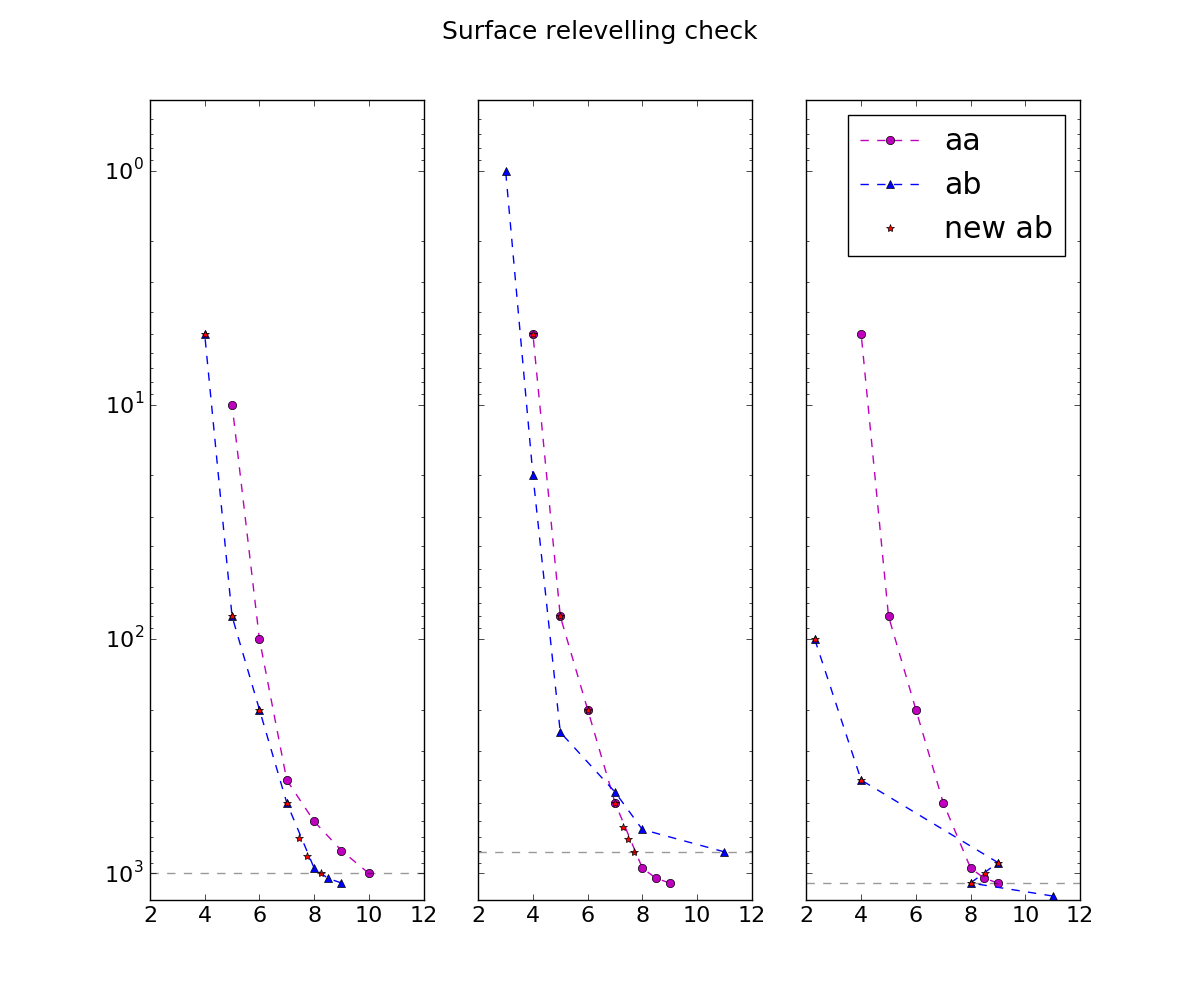
\includegraphics[width=\textwidth]{Figures/HCHO/SurfaceRelevelCheck.png}
      \caption{Constructed example of the initial interpolation of OMI's $\omega$ onto a pressure dimension with mismatched surface pressure.}
      \label{ch_HCHO:fig:AMF_Surface_Relevel}
      \end{figure}
      
      %If I change this to use an inverted geometric midpoint calculation then I need to explain it, otherwise I will need to note the assumption
      %$ \sqrt{ \left( P_1 \times P_{surf} \right)} = P_0 $
      %becomes $ P_{surf} = \frac{P_0^2}{P_1} $ where currently I'm using $P_0$ as the surface.
      
      S$_\sigma(\sigma)$ Is determined after running GEOS-Chem, which outputs vertical profiles of air density and HCHO mixing ratio, at 72 vertical levels with associated metadata such as vertical layer height and pressure, grid box location, height, and surface pressure.
      Using these outputs the vertical columns ($\Omega_a, \Omega_v$) are calculated for each horizontal grid point (i, j) as follows:
      \begin{align*}
      \Omega_a(i,j) &=& \Sigma_z \left( N_a(i,j,z) \times H(i,j,z) \right)
      \\
      \Omega_z(i,j) &=& \Sigma_z \left( N_{HCHO}(i,j,z) \times H(i,j,z) \right)
      \end{align*}
      where $N_a$, and $N_{HCHO}$ are the densities of air and HCHO, H is the layer height (for each grid box).
      Note that HCHO density is determined from the outputted mixing ratio: $N_{HCHO} = C_{HCHO} \times N_a$.
      
      S$_\sigma(\sigma)$ is then stored in HDF-EOS5 format, to be used in conjunction with the satellite measurements to calculate an AMF as shown in equation \ref{ch_HCHO:eqn:AMFintwSdz}.
      As the GEOS-Chem V10.01 output is in bitpunch format, the code to read the data and create the shape factor is written in IDL, which has many procedures and functions which are already written to handle reading this format (provided by GAMAP).
      The code is provided in supplementary TODO: put code into supplement section.
      
      For each OMI slant column, a new AMF is calculated using S$_\sigma(\sigma)$ and the provided scattering weights $\omega(\sigma)$ using equation \ref{ch_HCHO:eqn:AMFintwSdz}.
      This integral is applied in python by taking the sum of S$_\sigma(\sigma) \times \omega(\sigma) \times \mathrm{d}\sigma$ for each $\sigma$ determined at 72 levels in GEOS-Chem, with the provided $\omega$ interpolated linearly to these same levels.
      An example of these interpolations is shown in figure TODO: interpolation figure with symbols at original points and interpolated line overplotted for both functions over hPa.
      Globally this reprocessing changed the AMF by TODO: global total percent difference in AMF. 
      In total this caused TODO: total column HCHO change globally/yearly
      In Summer over Australia the global AMF difference was TODO: Difference summers only.
      This changed Australia's HCHO amounts from TODO: X to Y Tg per year plus minus one std.  
    
    
  \subsection{Old Fire Product MYD14C8H}
    % This stuff is no longe used - now using MOD14A1 gridded
    
    On board NASA's AQUA satellite, the MODIS instrument is used to detect fire activity.
    The product used here is called MYD14C8H (\parencite{Giglio2006}), which looks at fire activity over eight days on a 0.5$^{\circ}$ square grid globally.
    Regridding the product to the native meteorological grid of GEOS5 at 0.25$^{\circ}$ latitude by 0.3125$^{\circ}$ longitude is done in python with an interpolator which maps the values of the new grid rectangles to the value of the nearest grid square.
    
    Figure \ref{ch_HCHO:fig:fireexclusionexample} shows an example of the total column HCHO calculated using GEOS-Chem aprioris ($\Omega_{GEOS}$) before and after using the MYD14C8H product to exclude fire influenced pixels.
    (TODO: show time series of how many pixels are removed and discuss if this causes any issues down the line)
    % January 1, 2005 : 113384 / 130295 nan entries before and after fire exclusion within 60 degrees of equator
    
    \begin{figure}[!htbp]\begin{center}
      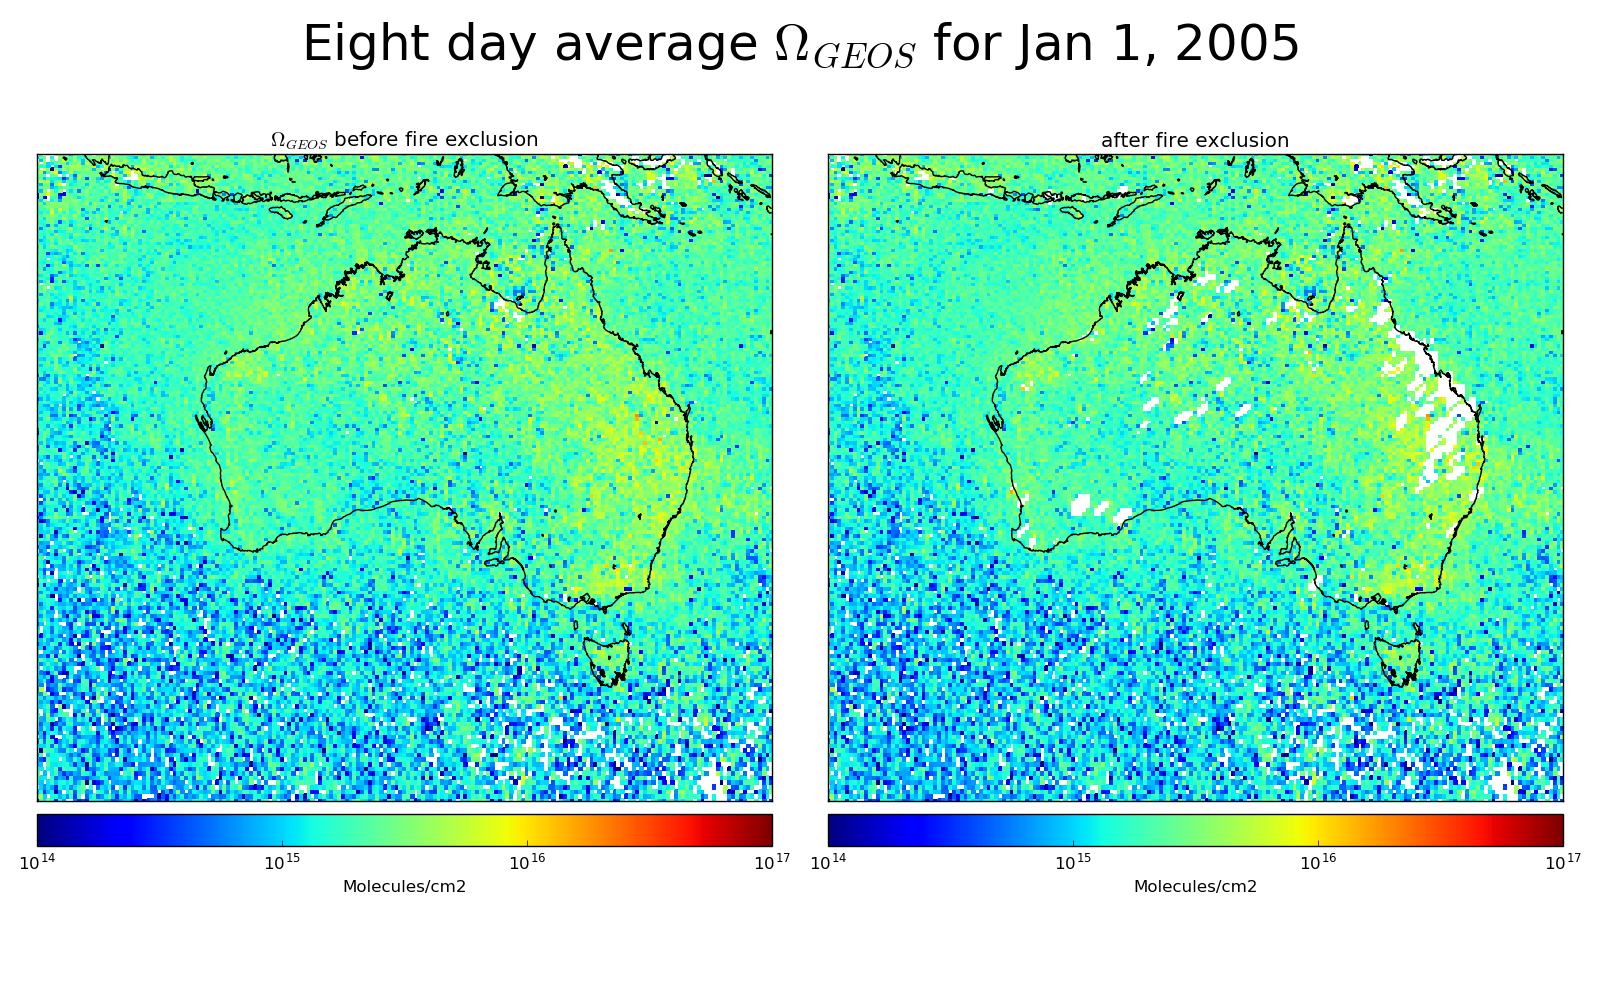
\includegraphics[width=\textwidth]{Figures/HCHO/fire_exclusion_aus_8d.png}
      \caption{Vertical column HCHO calculated using OMI satellite swaths with GEOS-Chem aprioris, averaged over 1-8 January 2005 with and without fire affected squares removed.}
      \label{ch_HCHO:fig:fireexclusionexample}
    \end{center}\end{figure}
      
    This filtering ends up removing too much information, and the recalculation of HCHO is too negatively influenced.
    To deal with this a separate product from the same instrument has been downloaded: MYD14A1, which keeps daily fire counts.
    Less disruptive filtering can be achieved by removing pixels which coincide with fires on the same day, as shown in figure TODO: which compares the 8 and 1 day filtering.
    TODO: The script to read and regrid these one day fire counts was adapted from X.
    Figure (TODO: effect on uncertainty and time series of fire pixels removed) shows the daily filtering effect on uncertainty and time series of fire pixels removed.
    
    An example of the change in resolution is provided in figure \ref{ch_HCHO:fig:modisgridspace}, where the grids are shown over a basic map of Tasmania.
    The direct affect of this interpolation is shown as an example in figure \ref{ch_HCHO:fig:modisinterpolation}, which is showing the regridded MODIS fire count over Australia from January 2005 (avg of first 8 days) in two subplots.
    
    \begin{figure}[!htbp]\begin{center}
        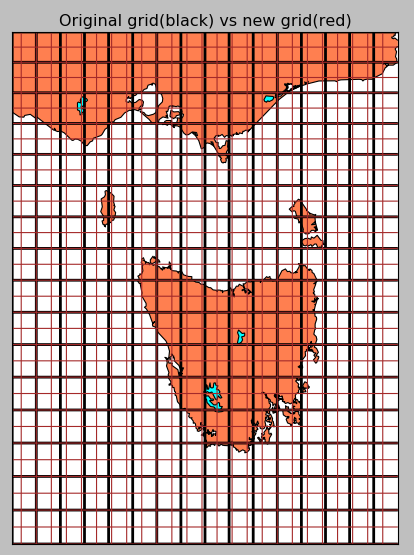
\includegraphics[width=0.7\textwidth]{Figures/MODIS_grid_space.png}
        \caption{Example of grid space change using 0.5x0.5 and 0.25x0.3125 latitude by longitude resolution.}
        \label{ch_HCHO:fig:modisgridspace}
      \end{center}\end{figure}
      
      \begin{figure}[!htbp]\begin{center}
          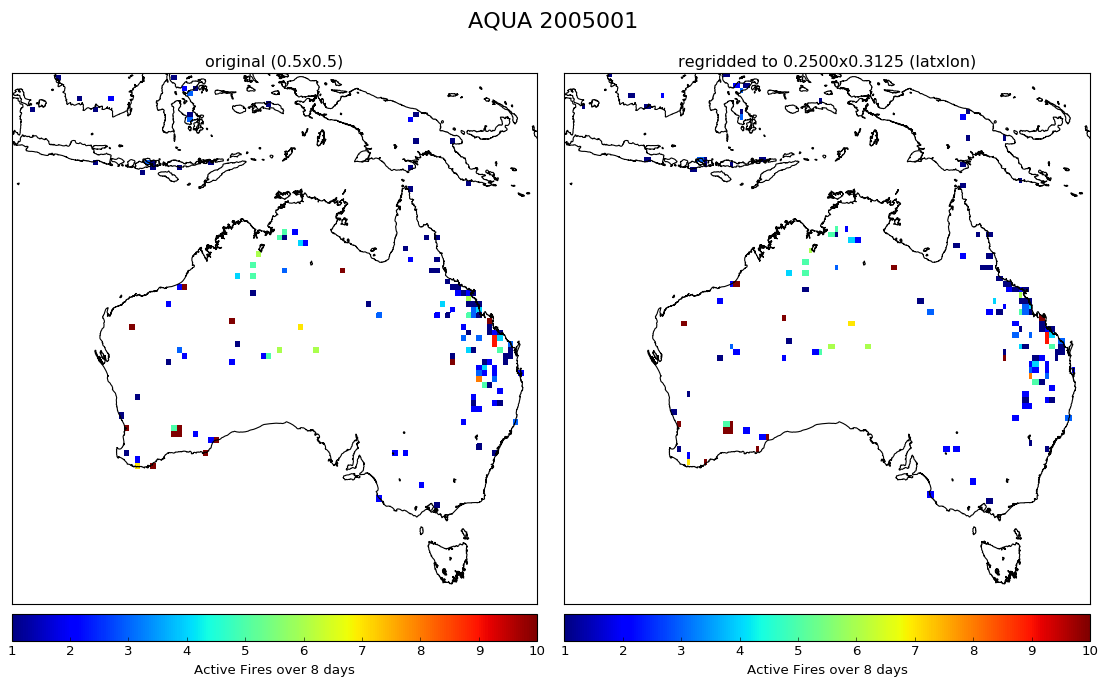
\includegraphics[width=\textwidth]{Figures/MODIS_Regrid_Comparison.png}
          \caption{Example of MODIS 8 day grid interpolation from 0.5x0.5 to 0.25x0.3125 latitude by longitude resolution.
            This example uses MODIS fire counts for 1-8 January 2005.}
          \label{ch_HCHO:fig:modisinterpolation}
        \end{center}\end{figure}